\section{Experiment Setup}\label{sec:replication} 
In this section we will introduce the setup of the experimental evaluation performed by the authors of the PGExplainer. While replicating their evaluation, we found that a number of steps were making assumptions that were not well documented. This includes the samples used for calculating the AUC score. In this section we will spend time on these steps. Additionally, some minor mistakes made in the original evaluation were rectified during our reproduction. These changes will also be highlighted here.

The experimental setup used by the authors of the PGExplainer follows that of the GNNExplainer \cite{ying2019gnnexplainer} with a number of extensions. To clarify, the authors' proposed method serves the purpose of explaining the classification decision of a GNN. Hence, the experiments used to evaluate the PGExplainer focus on the explanations provided by the PGExplainer for the underlying model. Specifically, the evaluation is repeated for six different datasets, and thus, for six different underlying models. The six datasets span two different classification tasks; node-classification and graph-classification. 

\subsection{Datasets \hfill \texttt{[datasets/dataset\_loaders.py]}}\label{sec:datasets}
The node classification task is performed using four synthetic datasets (a-d). All of which are first introduced in the GNNExplainer paper \cite{ying2019gnnexplainer}. The graph classification task is performed using two datasets (e-f), one synthetic and one real.

A reoccurring concept in all synthetic datasets is the so called \textit{motif}. Motifs are highly structured subgraphs---e.g. 9 nodes connected in a 2D grid. These subgraphs are then expanded by attaching them to a randomly generated graph of a different structural form---e.g. Barabasi-Albert (BA) graph \cite{Barabasi99emergenceScaling} or trees. Motifs play a crucial role in determining ground-truth explanations for our evaluations, as we will see later.
% All six datasets are specified and visualised in Table \ref{tab:results} (Appendix \ref{appendix:A}) \cite{luo2020parameterized}.

(a) The BA-Shapes dataset consists of single base BA-graph with 300 nodes, 80 “house”-structured motifs---each attached to random BA nodes---and some extra randomly added edges. (b) BA-Community closely resembles BA-Shapes, connecting two BA-Shapes and utilizing a Gaussian distributions for each BA-Shape to sample node features. (c) Tree-Cycles adopts an $8$-level balanced binary tree as the base graph with a set of $80$ six-node cycle motifs attached to randomly selected nodes. (d) The Tree-Grids dataset is similar to Tree-Cycles, replacing cycle motifs with $3\times 3$ grid motifs. (e) The authors constructed the BA-2motifs dataset consisting of $1000$ BA graphs. Half of the graphs contain "house" motifs, the other half contain five-node cycle motifs attached to the BA graph. These two types of graphs serve as the two classes for the dataset. (f) The real-life Mutagenicity dataset copied from \cite{ying2019gnnexplainer}, consisting of $4337$ molecule graphs. These should be classified as either mutagenic or nonmutagenic.
% All base nodes are labelled $0$, the nodes constructing the "house"'s top, middle and bottom are labelled $1$, $2$ and $3$ respectively. 
% In BA-Community nodes are labeled based on their structural roles and community memberships, leading to $8$ classes in total.


% \begin{enumerate}[(a)]
%     \item The BA-Shapes dataset consists of single base Barabasi-Albert (BA) graph \cite{Barabasi99emergenceScaling} with 300 nodes, 80 “house”-structured motifs---each attached to random BA nodes---and some extra randomly added edges. All base nodes are labelled $0$, the nodes constructing the "house"'s top, middle and bottom are labelled $1$, $2$ and $3$ respectively. 
%     \item BA-Community closely resembles BA-Shapes, connecting two BA-Shapes and utilizing a Gaussian distributions for each BA-Shape to sample node features. In BA-Community nodes are labeled based on their structural roles and community memberships, leading to $8$ classes in total.
%     \item Tree-Cycles adopts an $8$-level balanced binary tree as the base graph with a set of $80$ six-node cycle motifs attached to randomly selected nodes.
%     \item The Tree-Grids dataset is similar to Tree-Cycles, replacing cycle motifs with $3\times 3$ grid motifs.
%     \item The authors constructed the BA-2motifs dataset consisting of $1000$ BA graphs. Half of the graphs contain "house" motifs, the other half contain five-node cycle motifs attached to the BA graph. These two types of graphs serve as the two classes for the dataset.
%     \item The real-life Mutagenicity dataset copied from         \cite{ying2019gnnexplainer}, consisting of $4337$ molecule graphs. These should be classified as either mutagenic or nonmutagenic.
% \end{enumerate}


% In order to compare and evaluate results, the authors use the four datasets found in \cite{ying2019gnnexplainer}; BA-Shapes (1), BA-Community (2), Tree-Cycles (3), and Tree-Grids (4). Additionally, they construct a fifth graph classification dataset, BA-2motifs (5). All five datasets are also specified and visualised in Table \ref{tab:dataset_info} and Table \ref{tab:results} \cite{luo2020parameterized}.
% (1) The BA-Shapes dataset consists of single base Barabasi-Albert (BA) graph \cite{Barabasi99emergenceScaling} with 300 nodes, 80 “house”-structured motifs---each attached to random BA nodes---and some extra randomly added edges. All base nodes are labelled $0$, the nodes constructing the "house"'s top, middle and bottom are labelled $1$, $2$ and $3$ respectively. 
% (2) BA-Community closely resembles BA-Shapes, connecting two BA-Shapes and utilizing a Gaussian distributions for each BA-Shape to sample node features. In BA-Community nodes are labeled based on their structural roles and community memberships, leading to $8$ classes in total.
% (3) Tree-Cycles adopts an $8$-level balanced binary tree as the base graph with a set of $80$ six-node cycle motifs attached to randomly selected nodes.
% (4) The Tree-Grids dataset is similar to Tree-Cycles, replacing cycle motifs with $3\times 3$ grid motifs.
% (5) The authors constructed the BA-2motifs dataset consisting of $1000$ BA graphs. Half of the graphs contain "house" motifs, the other half contain five-node cycle motifs attached to the BA graph. These two types of graphs serve as the two classes for the dataset.
% (6) Finally, they include the real-life MUTAG dataset copied from \cite{ying2019gnnexplainer}, consisting of $4337$ molecule graphs. These should be classified as either mutagenic or nonmutagenic.


% \begin{table}[h]
%     \centering
%     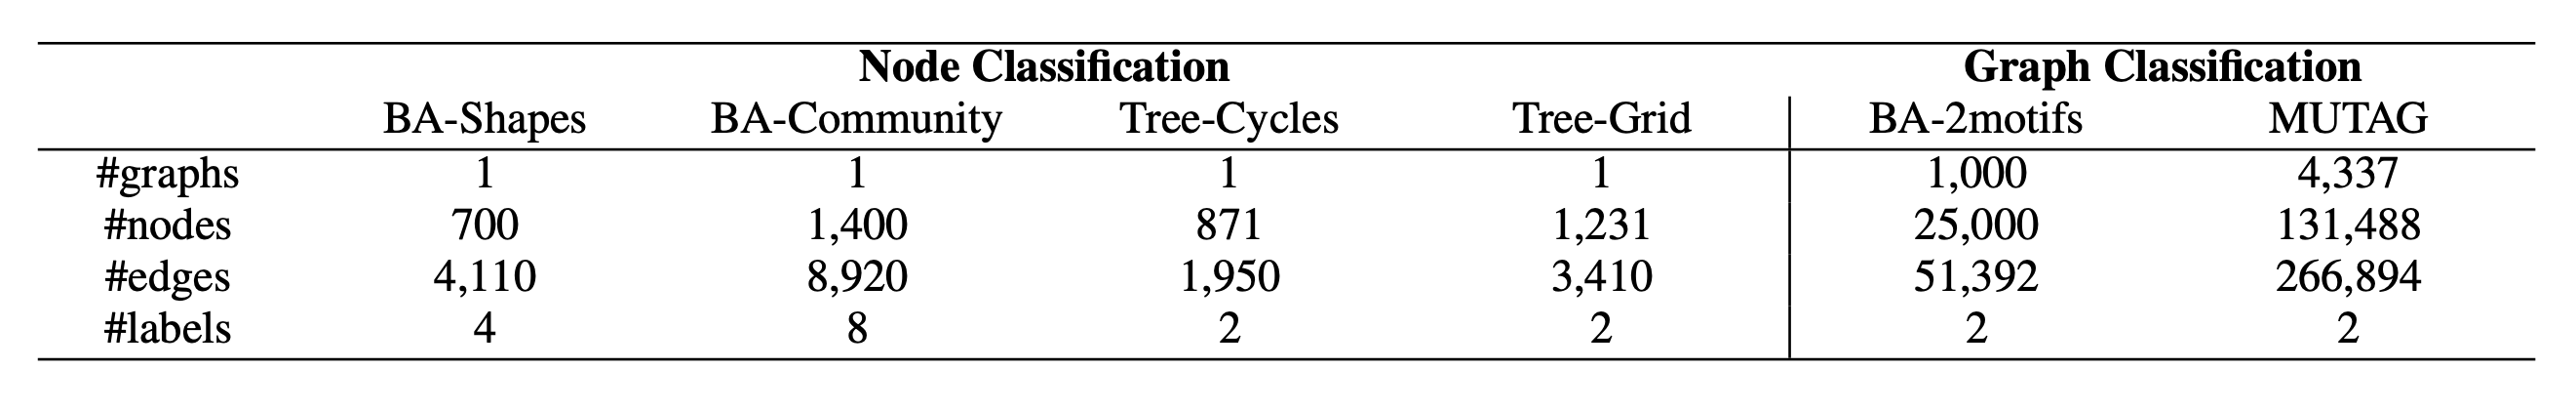
\includegraphics[width=1\linewidth]{imgs/dataset_info.png}
%     \caption{Original paper's dataset statistics \cite{luo2020parameterized}}
%     \label{tab:dataset_info}
% \end{table}

\subsection{Model \hfill \texttt{[models/GNN\_paper.py]}}
There are a number of large differences between the implementation of the models trained for each dataset and how they are described in the paper. These changes are different between the node and graph classification tasks. 

\paragraph{Node classification}
The authors describe the model for node classification to be three consecutive Graph Convolution layers feeding directly into the fully connected classification. The model in the codebase however first concatenates the three intermediate outputs of the Graph Convolution layers before using this enlarged embedding as the input for the fully connected classification layer. The coded version of the models is similar to what is used for evaluation in the GNNExplainer paper \cite{ying2019gnnexplainer}. To keep the evaluation consistent, we will therefore use the coded model version instead of the one described in the paper for our evaluation. Moreover, we were not able to get the model described in the paper to train to the same accuracy using the provided hyperparameters. 

In addition to the architecture change, we found the node classification models to use an undocumented batch normalization layer after the first and second Graph Convolution layer. Unfortunately, the original codebase contained an error that resulted in these batch-normalization layers being kept in training mode during evaluation. This observation was confirmed by the authors in communication and has since been resolved. In the same communication the authors expressed that to be able to reproduce their results, the batch normalization layers will have to be kept in training mode. We believe that this will compromise the usability of our reproducibility experiment and therefore decided to remove the batch normalization layers all together. For completeness full replication of the authors evaluation with a model containing batch normalization is included in Appendix \ref{appendix:batch_norm}.

\paragraph{Graph classification}
The graph classification models are more in line with the models described in the paper than the node classification models. The difference is the use of both max and mean pooling over the output of the final Graph Convolution layer. These two pooling types are concatenated to form inputs for fully connected layers.  

% In contrast to what is described in the paper, the model for which the PGExplainer provides explanations is considerably different from the model used in the GNNExplainer paper. Most notably, the authors included additional batch normalization layers for the first and second Graph Convolution layer. In addition to this, the implemented model does also not follow the general model structure as defined in the paper. Instead of using consecutive 3 Graph convolution layers feeding directly into the fully connected classification layer, the coded model first concatenates the three outputs of the GC layers before feeding it. 

% - Describe the model that they implemented in their code
%     - same as GNNExplainer, with additional batch normalization
% - In contrast to what is defined in the paper, the layers are concatenated
% - Use of both max and mean pooling in code, but not paper
% \paragraph{Training}
%     - As described in paper
%     - Main difference in code is longer training of the Graph classification models

\subsection{Evaluation metrics \hfill \texttt{[tasks/replication.py]}}

For each dataset, the explanations are evaluated using three broad categories; quantitative, qualitative and efficiency.

\subsubsection{Quantitative evaluation \hfill \texttt{[evaluation/AUCEvaluation.py]}}
For each dataset the explanations provided by the PGExplainer are compared to ground-truth explanations. These ground-truths describe for each sample which edges should or should not be included in the explanation. Using this methodology, the quantitative evaluation can be performed similar to a binary classification task. For this reason, the authors present the quantitative score using the AUC scoring metric. 

\paragraph{Ground Truth }
For node classification the ground-truth explanation is determined globally---i.e. for all node samples the edges have the same ground-truth explanation label. Specifically, for each edge it is determined if the two nodes it connects are part of a motif. When this is the case, the edge is labelled as positive for the ground-truth explanation. Otherwise, the edge is labelled as negative for the ground-truth explanation. For graph classifications this is dependent on the dataset used and how the ground-truth explanations are generated. For the BA-2motif dataset, being synthetic, this is done the same way as for the node datasets. The only difference being that the process is repeated for every graph in the dataset. As there are no motifs defined for the Mutagenicity dataset, the ground-truth labels can not be defined based on them. Instead, for this dataset edge labels are used, as provided by the original dataset repository\footnote{https://ls11-www.cs.tu-dortmund.de/staff/morris/graphkerneldatasets}. 

\paragraph{AUC score}
With the explanation mask provided by the PGExplainer and the ground-truths defined as above, the AUC score can be computed. However, there are a few important notes to consider when computing the AUC score. First, for the node classification datasets, the explanation mask is only determined for a 3-hop graph around each node. This is done because the GCN model only contains three layers. Second, only the nodes that are part of a motif are used in the AUC computation. This is because there is no real definition of ground-truth for the nodes outside the motifs. This evaluation design choice is further discussed in Sec.\,\ref{sec6}. Third, for the BA-2Motif dataset only a subset of the graphs is used to determine the AUC score, this is done to reduce computation time. Lastly, for the Mutagenicity dataset only the mutagenic graphs have a valid ground-truth interpretation. Hence, the AUC is determine using only these graphs. Of these four considerations, only the last is mentioned in the original paper. 

\paragraph{Comparison} The authors compare their method against four baselines; a gradient-based model (GRAD) \cite{ying2019gnnexplainer}, a graph attention network (ATT) \cite{velivckovic2017graph} and Gradient \cite{pope2019explainability}. With the exception of the scores presented for the graph-classification datasets, the scores presented are reused from the PGExplainer paper (see Table \ref{tab:results}). In communication with the authors, it was mentioned that the reimplementation of these explainers by the authors had resulted in lackluster results. For this reason the decision was made to use the original scores by the original authors. 

For our replication of the evaluation we focus our comparison on the GNNExplainer. This method is the most similar and was a major inspiration for the PGExplainer. In contrast the the original evaluation, we do perform the comparison using our own re-implementation of the GNNExplainer. Our re-implementation of this method is largely inspired by the implementation in the PyTorch Geometric library. The main difference is that our re-implementation is adapted to also work with graph-classification datasets. This is not possible with the plain PyTorch Geometric implementation. 

\subsubsection{Qualitative evaluation \hfill \texttt{[utils/plotting.py]}}
In order to obtain a visualisation of the chosen sub-graph the system takes as input the ground truth labels and the mask provided by the Explainer. Given the mask, two thresholds are calculated, one for importance to the explanation and one to determine which other elements to plot for the sub-graph. Then, using these thresholds all nodes that have an interesting enough weight are selected. Following this, only nodes that are in a direct sub-graph together the node-to-be-explained are selected. When drawing the explanation for the graph classification this sub-graph is selected using the top-$k$ edges. The original evaluation sets $k$ to be the number of edges in the defining motif for the synthetic datasets. These edges are plotted with a colour coding in accordance to their weight, where darker edges have higher weights in the mask than the lighter edges. Finally, the nodes that are connected to the previously plotted edges are plotted and colour coded by their ground-truth label.

\subsubsection{Efficiency evaluation \hfill \texttt{[evaluation/EfficiencyEvaluation.py]}}
In the paper, the authors only compare the efficiency of their PGExplainer to the GNNExplainer. Unfortunately, we were unable to extract the exact method for doing so from both the paper and the provided codebase. Our implementation is therefore mainly our own design.

We compute the inference time as the average over ten runs. During each run we measure the times it takes to explain all samples that are also used for the quantitative evaluation. This time is divided by the number of samples explained to get the final inference time per sample in milliseconds. Note that, similar to the paper, for the evaluation of the PGExplainer only the time to explain each sample is considered. On the other hand, for the GNNExplainer the time required to train the explainer is also taken into account because it has to be retrained for each sample. 

% The experimental settings closely follow those of the GNNExplainer \cite{ying2019gnnexplainer}. A three-layered GNN for each dataset is trained prior to explaining the predictions made by the GNN. 
% - Evaluation done on three levels, Qualitative, Quantitative and Inference
% - Using 2 different tasks, four datasets node classficiation and 2 datasets grap classification
% - Complete evaluation done using a single model
% \paragraph{Qualitative evaluation}
% - Single example presented for each dataset
% - Based on code the example is handpicked 
% \paragraph{Quantitative evaluation}
% - For each dataset a ground truth explanation is constructed
% - Ground truth describes for each edge if it should be included in th explanation or not. Based on this, the accuracy of the explanation can be calculated
% - Note that there are some important things to keep in mind for this way of evaluating
%     - for each dataset, a save set of nodes to perform the evaluation on is defined
%     - in case of node-classification, this is only the 3hop subgraph
%     - in case of graph-classification, this is the entire graph
% \paragraph{Efficiency evaluation}
% - Compare GNNExplainer vs. PGExplainer. Do not take into account training time for PGExplainer.
% - Different frameworks are used for both models and a different implementation style
% - No code included in the repo to reproduce this result. 

        

    
% \subsection{Results}
% \paragraph{Model training}
% In Tab.~\ref{tab:accuracies} the final accuracies of all models are provided. Note that these are the accuracies of the models that will be explained by the PGExplainer, not the explanation accuracies for the PGExplainer itself. For most models, using the configurations found in the code, we achieve results comparable to the results presented in the paper, except for the BA-Community and Mutagenicity models. 

% \begin{table}[]
% \centering
% \begin{tabular}{cccccccc}
% \toprule
% &\multicolumn{4}{c}{\textbf{Node Classification}} & \multicolumn{2}{c}{\textbf{Graph Classification}} \\
% Accuracy & \multicolumn{1}{c}{BA-Shapes} & \multicolumn{1}{c}{BA-Community} & \multicolumn{1}{c}{Tree-Cycles} & \multicolumn{1}{c|}{Tree-Grid} & \multicolumn{1}{c}{BA-2motifs} & \multicolumn{1}{c}{Mutagenicity} \\ 
% \midrule
% Training & 0.98 & 0.94 & 0.96 & \multicolumn{1}{c|}{0.96} & x.xx & 0.82 \\
% Validation & 0.99 & 0.74 & 0.99 & \multicolumn{1}{c|}{0.98} & x.xx & 0.82 \\
% Testing & 1.00 & 0.71 & 0.97 & \multicolumn{1}{c|}{0.99} & x.xx & 0.81 \\
% \bottomrule
% \end{tabular}
% \caption{Accuracies for models}
% \label{tab:accuracies}
% \end{table}

% %                 Node classification                         Graph classification
% %               Syn1, syn2m= .....                      Ba2, mutag
% % -----
% %visualization
% %------
% % PG them auc
% % PG us auc
% % ----
% % inference time
% \begin{table}[]
% \centering
% \begin{tabular}{lllllll}
% \toprule
% \multicolumn{5}{c}{\textbf{Node Classification}} & \multicolumn{2}{c}{\textbf{Graph Classification}} \\
% \multicolumn{1}{c}{} & \multicolumn{1}{c}{BA-Shapes} & \multicolumn{1}{c}{BA-Community} & \multicolumn{1}{c}{Tree-Cycles} & \multicolumn{1}{c|}{Tree-Grid} & \multicolumn{1}{c}{BA-2motifs} & \multicolumn{1}{c}{Mutagenicity} \\ \hline
% \multicolumn{7}{l}{\textbf{Visualization}} \\ \hline
% Original &  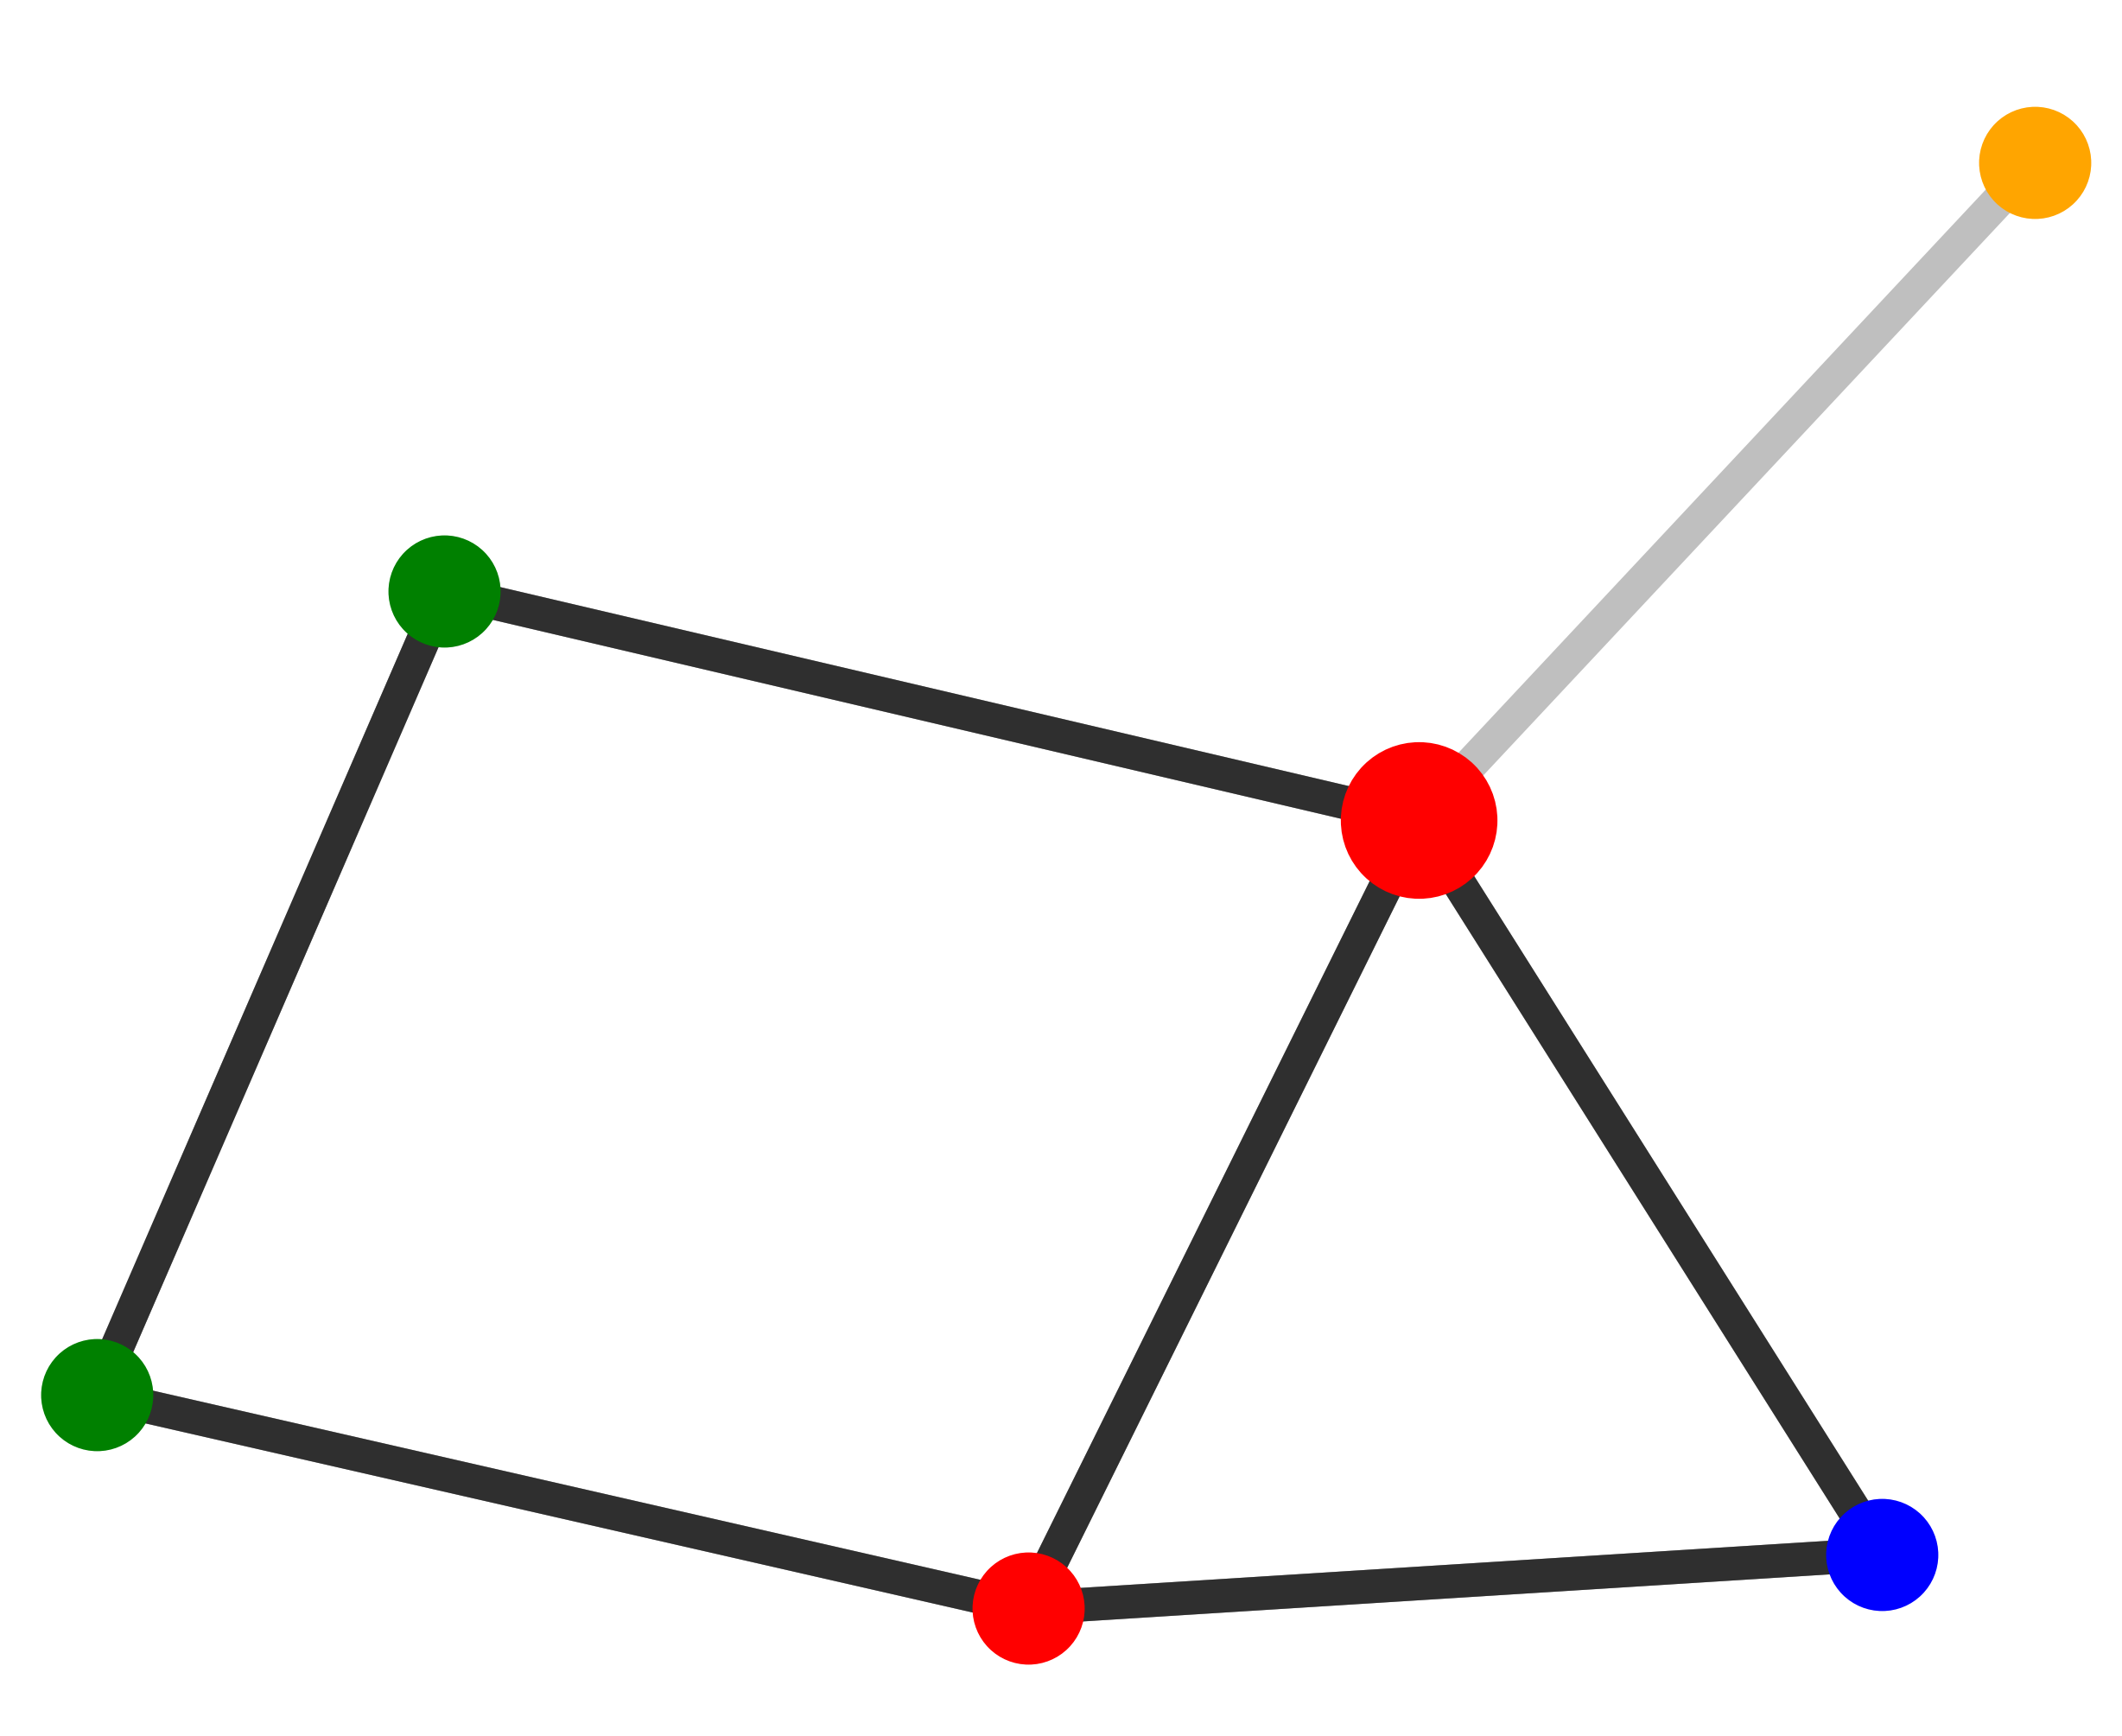
\includegraphics[width=.1\linewidth]{imgs/their_image-1.png}
% & 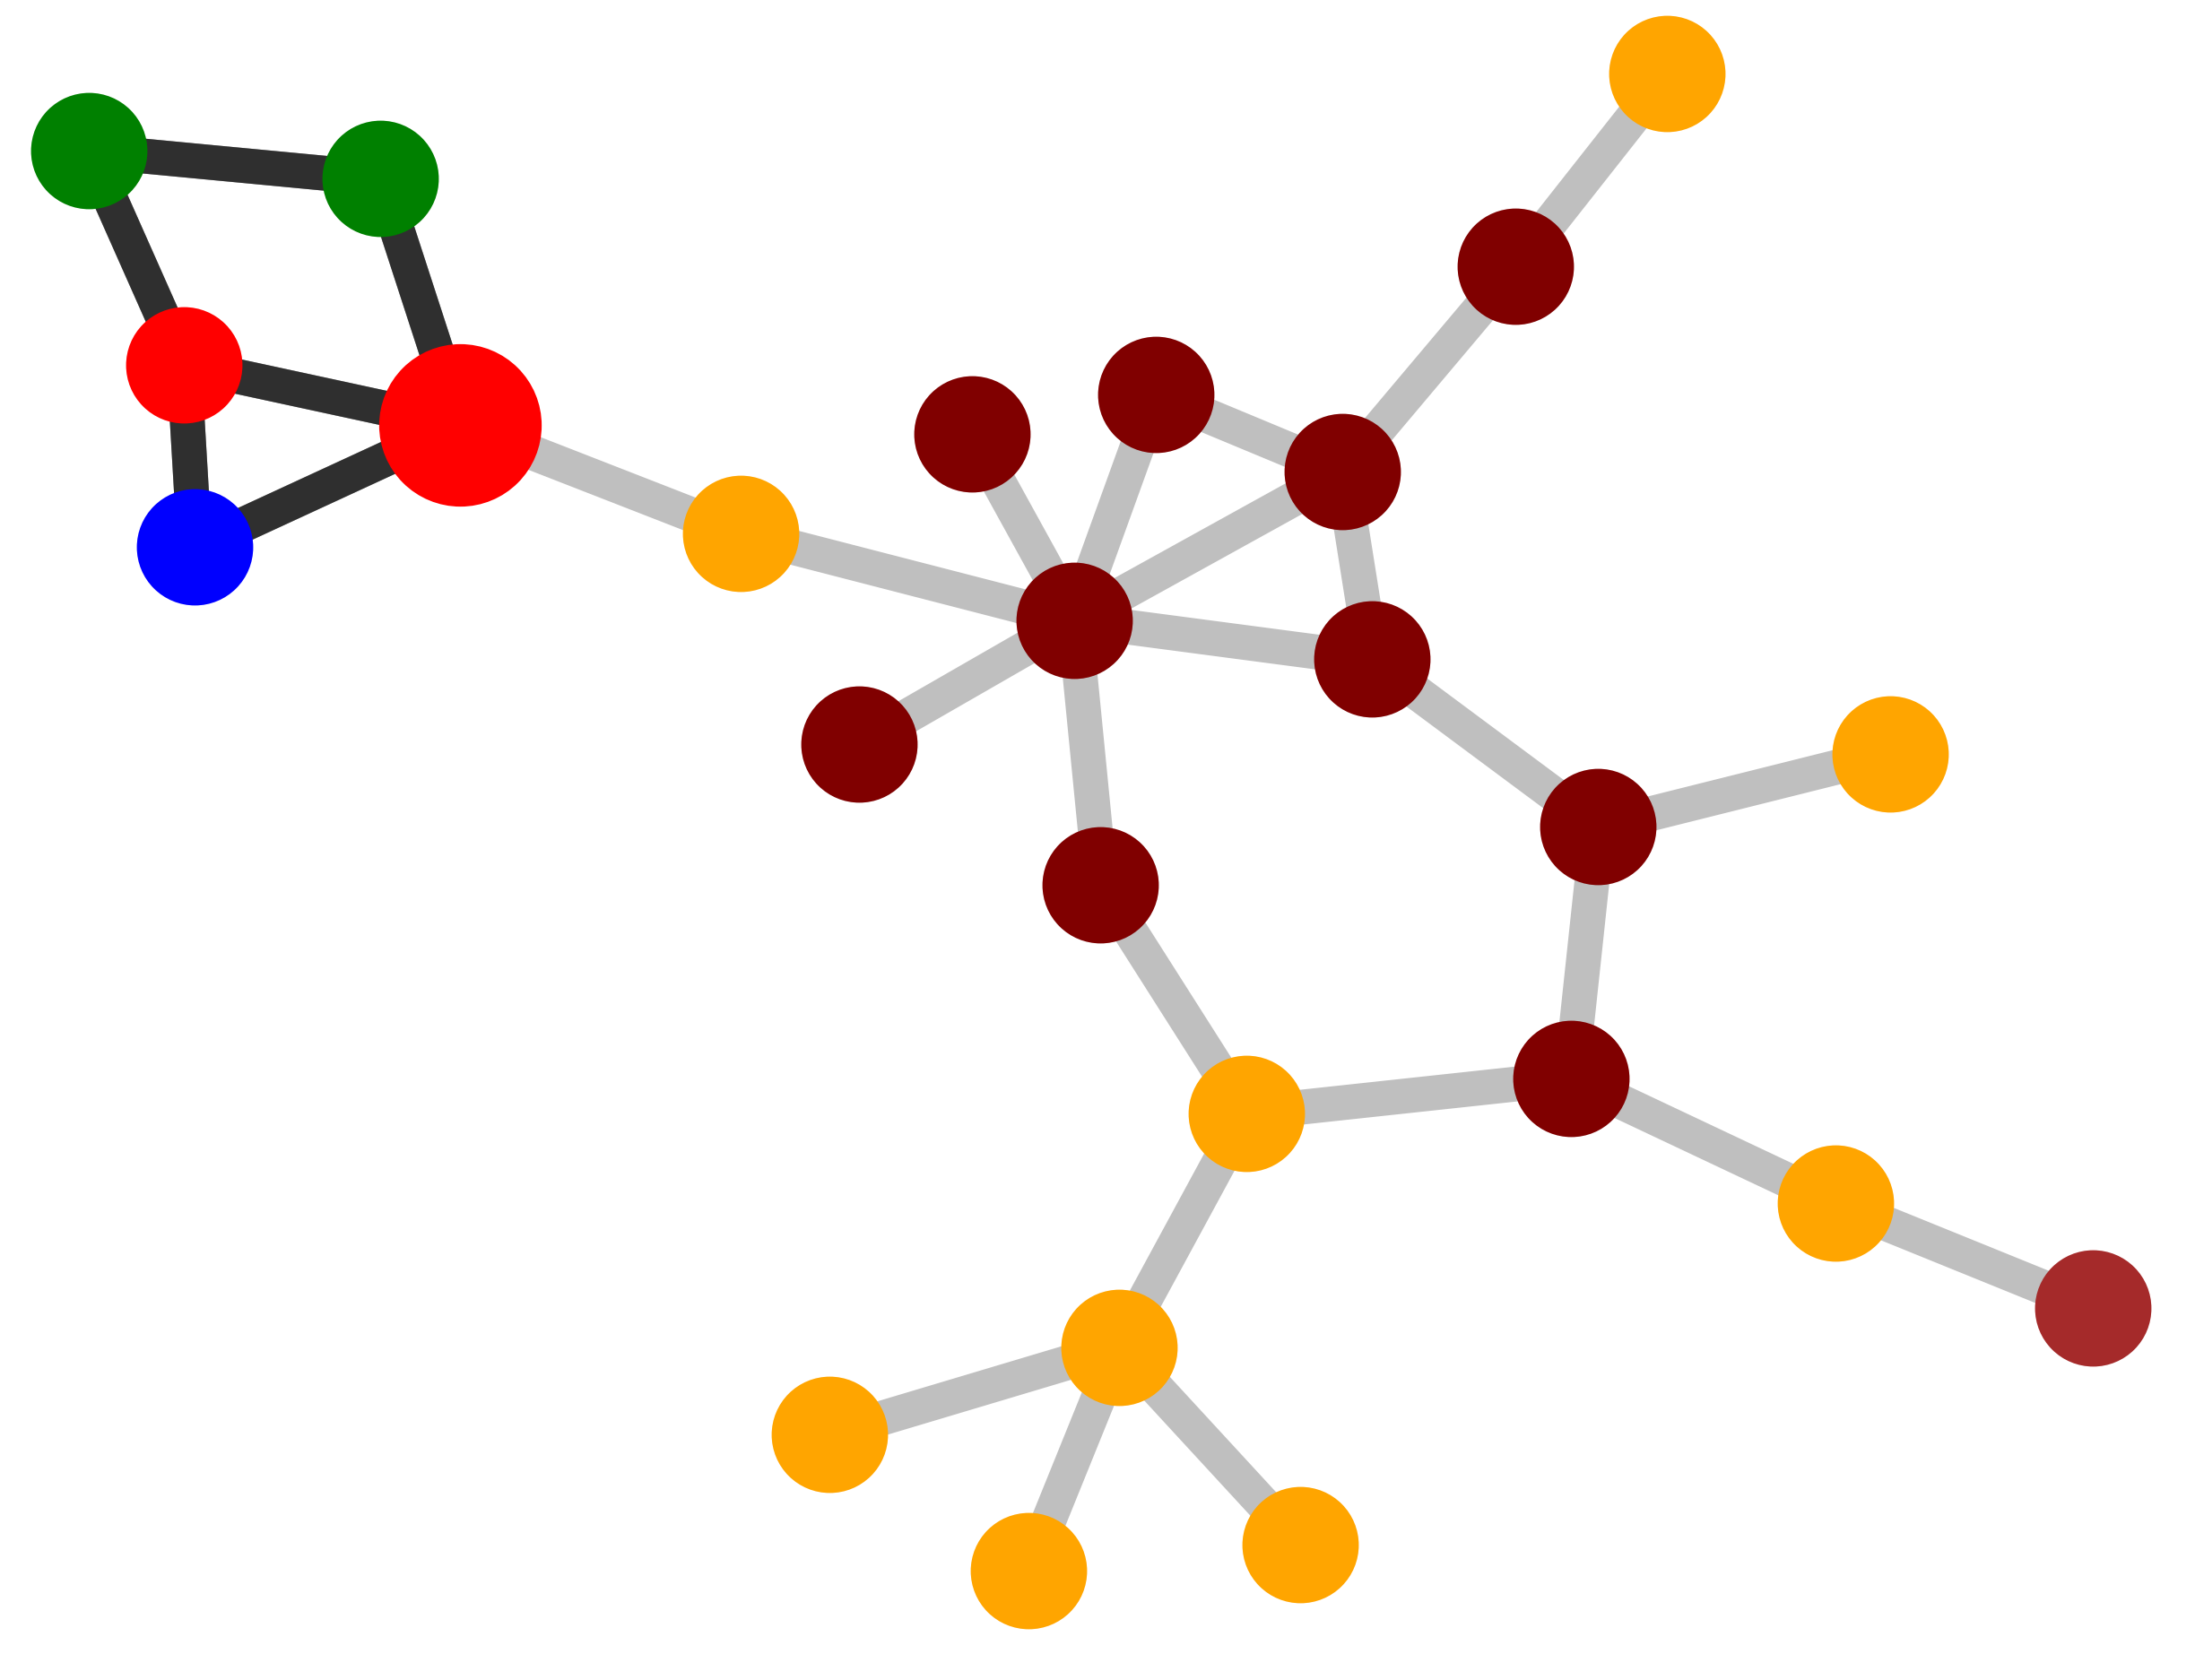
\includegraphics[width=.1\linewidth]{imgs/their_image-2.png} & 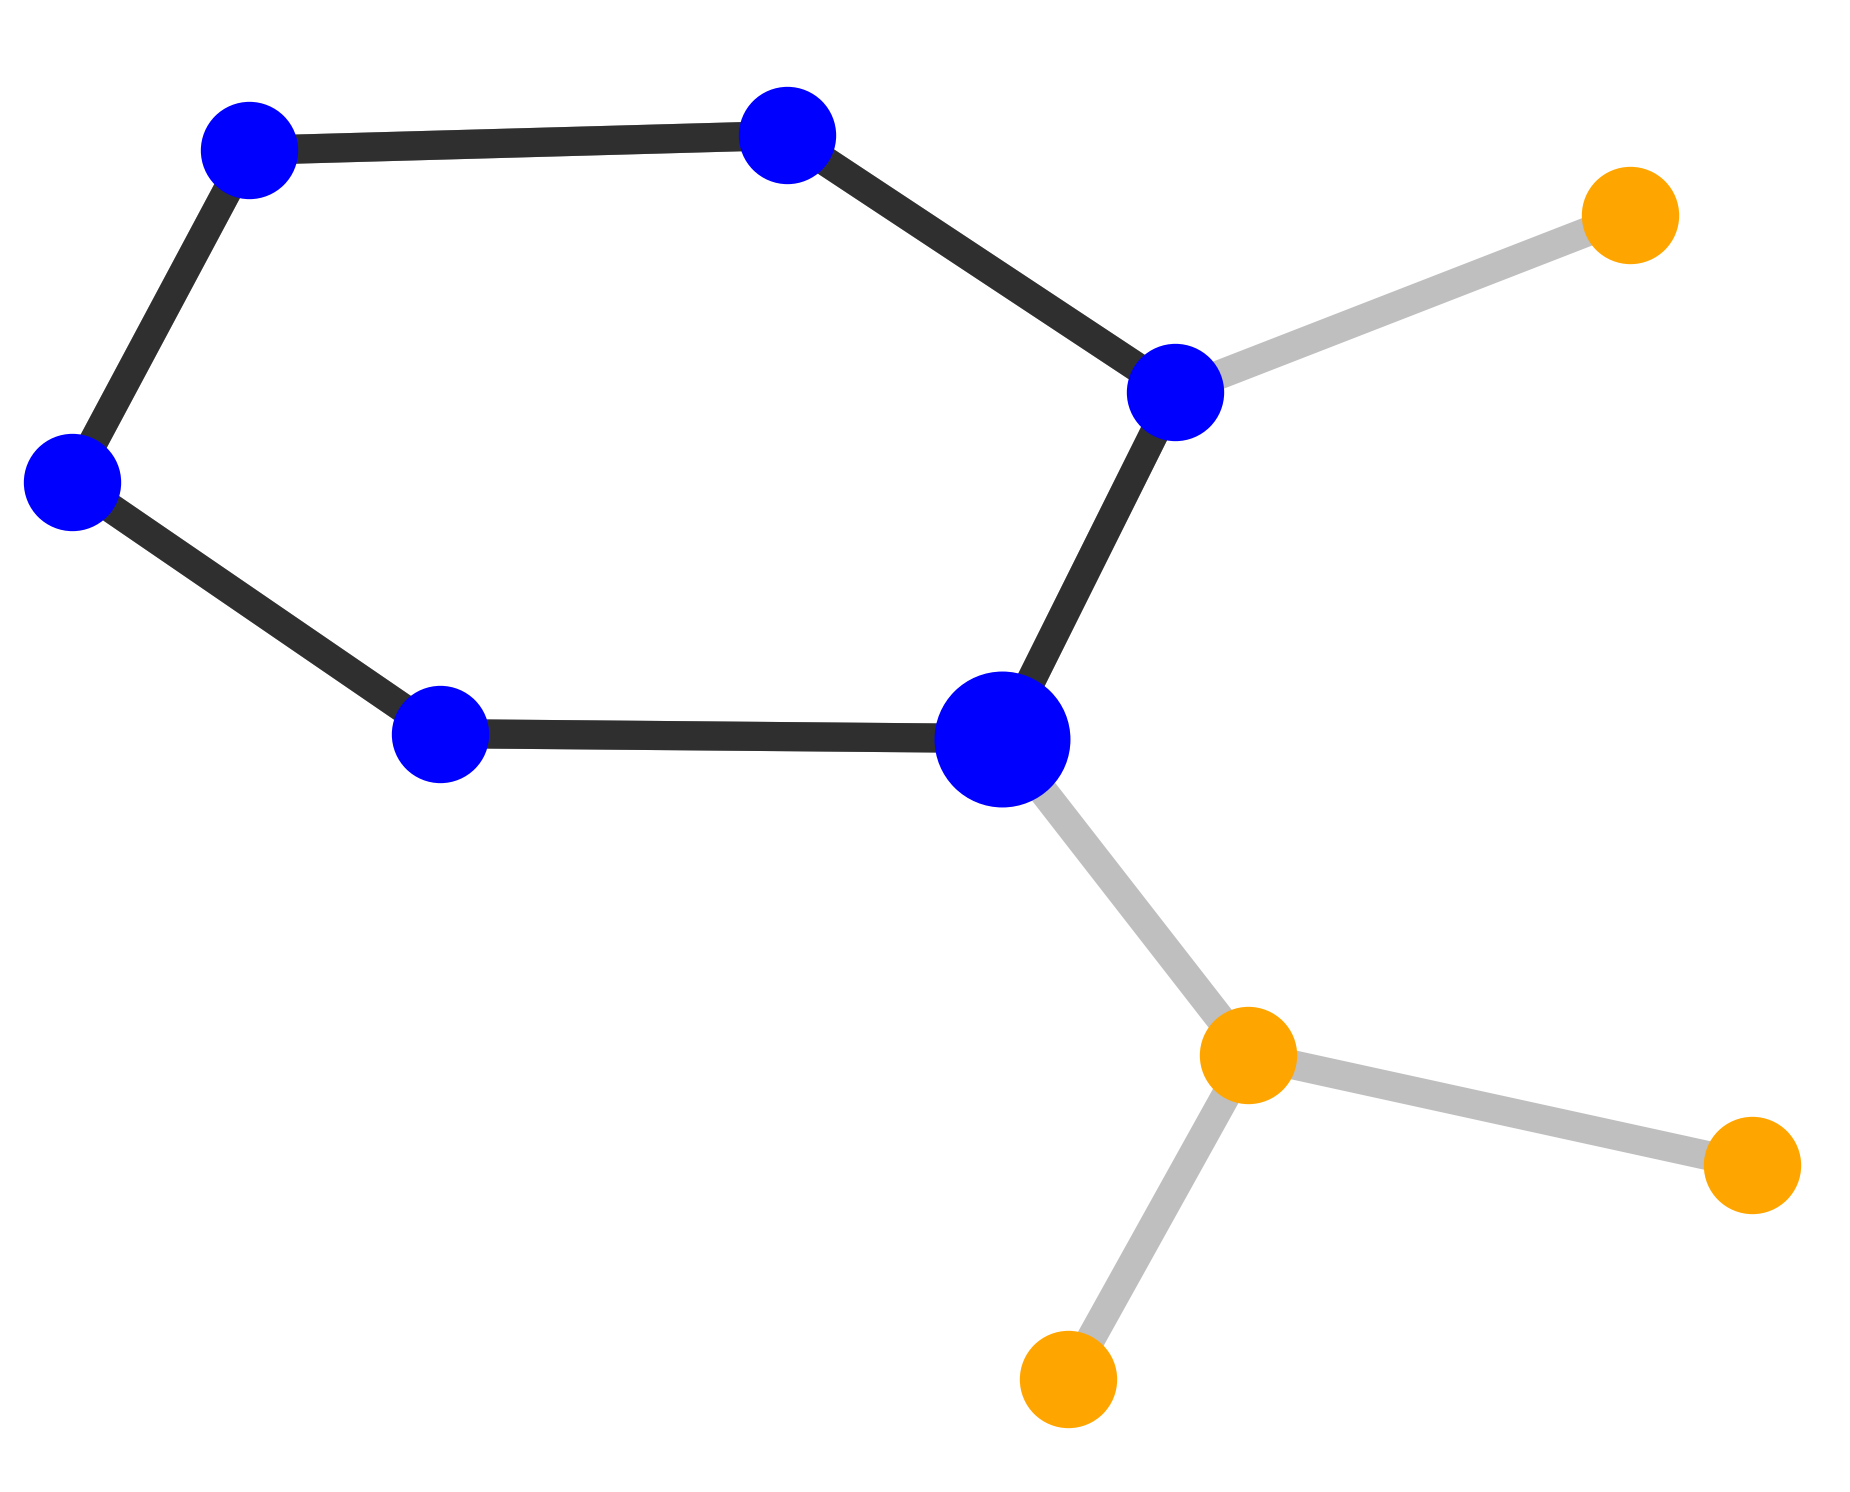
\includegraphics[width=.1\linewidth]{imgs/their_image-3.png} & \multicolumn{1}{l|}{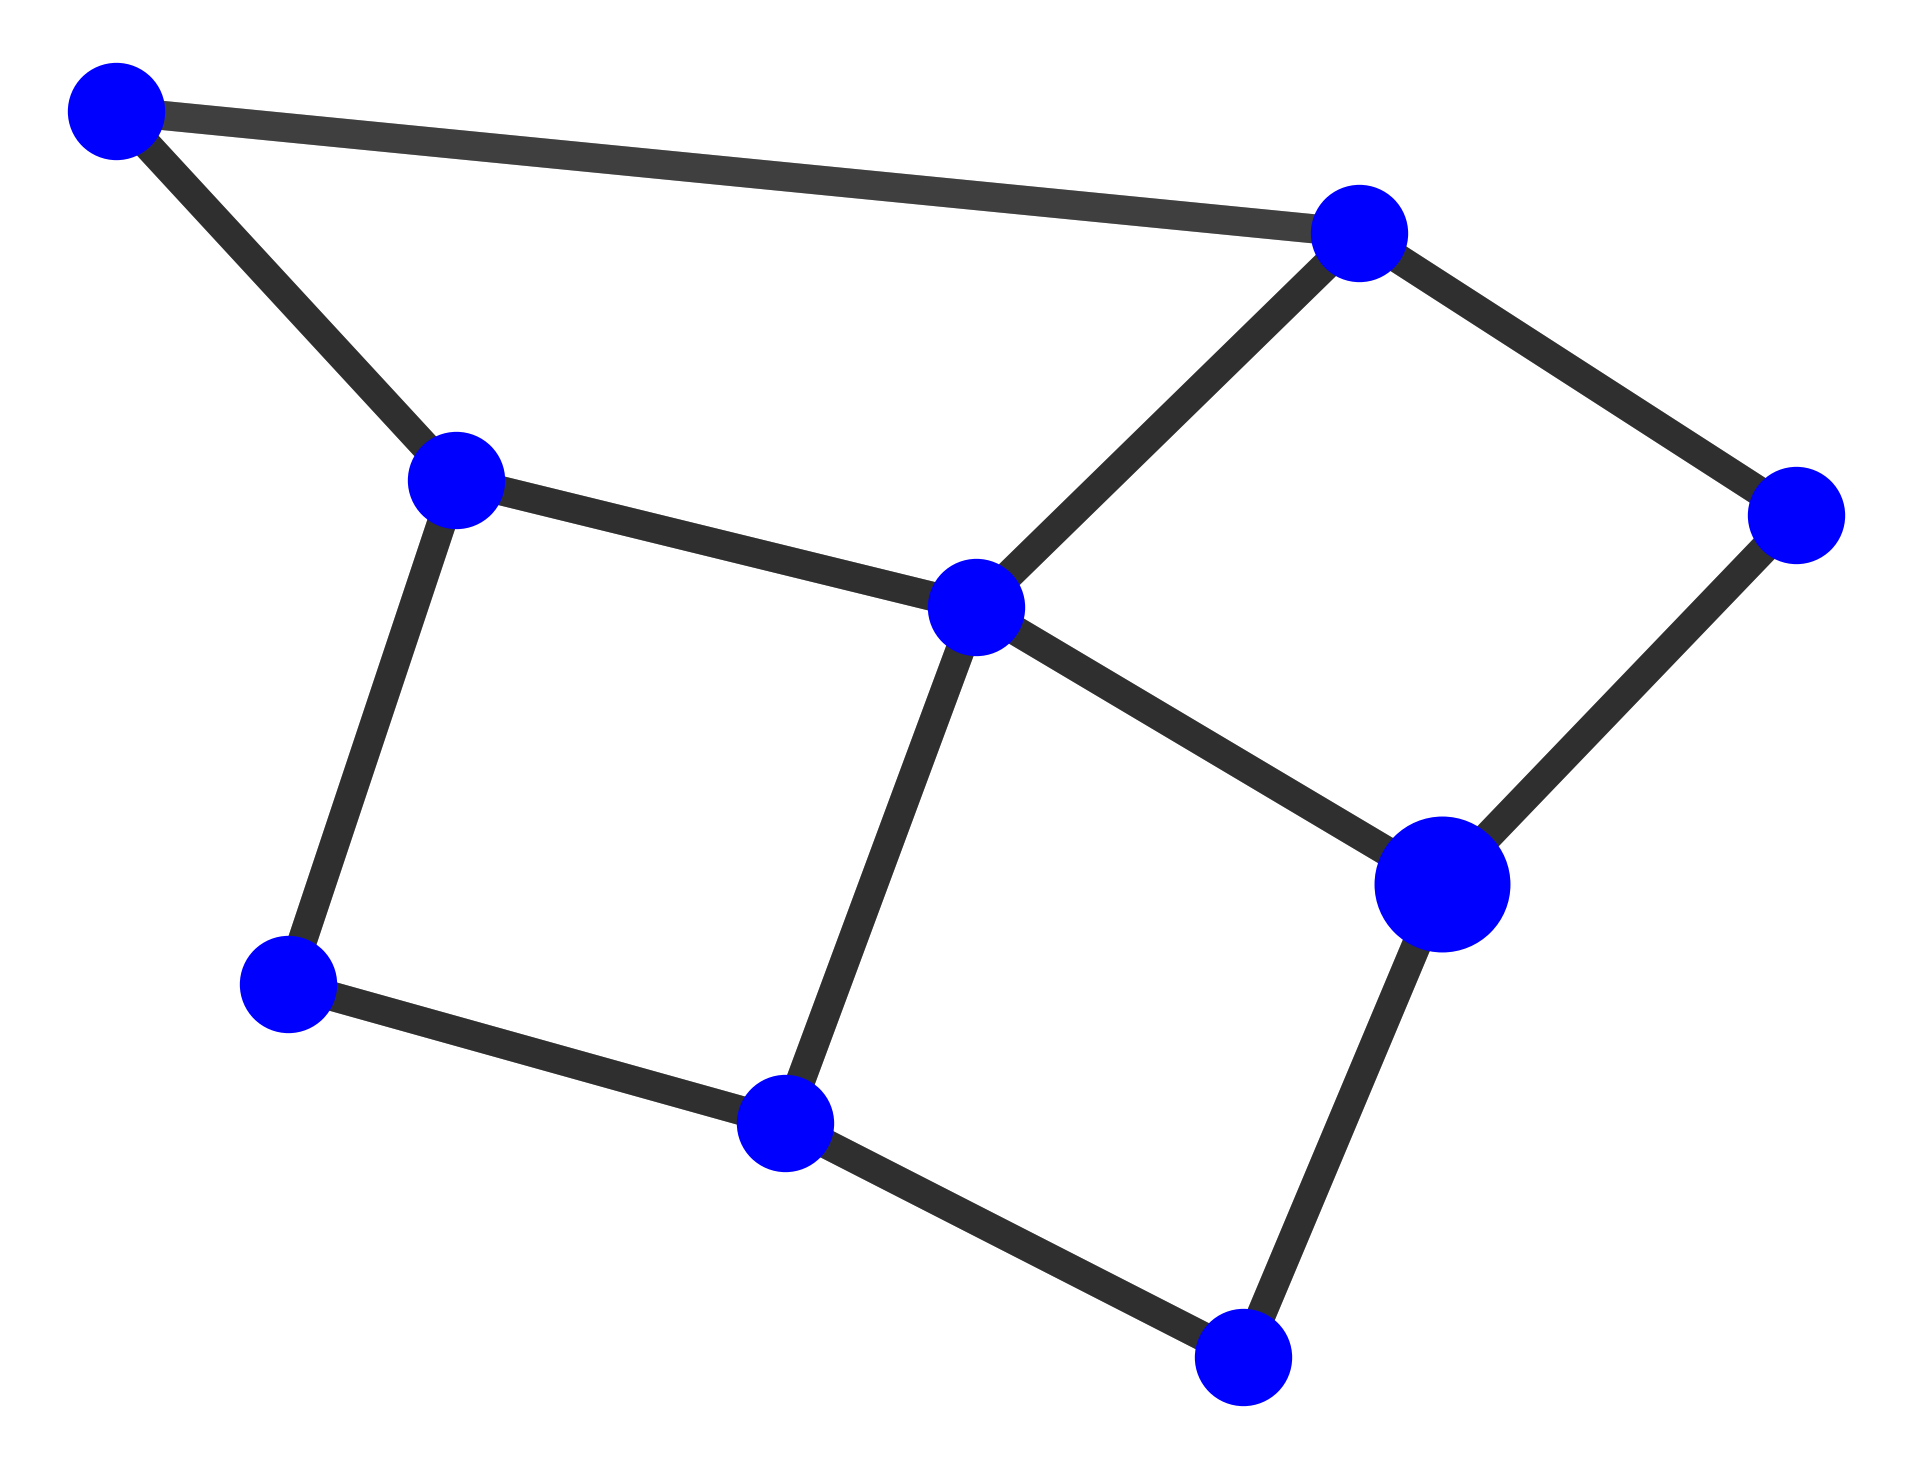
\includegraphics[width=.1\linewidth]{imgs/their_image-4.png}} & 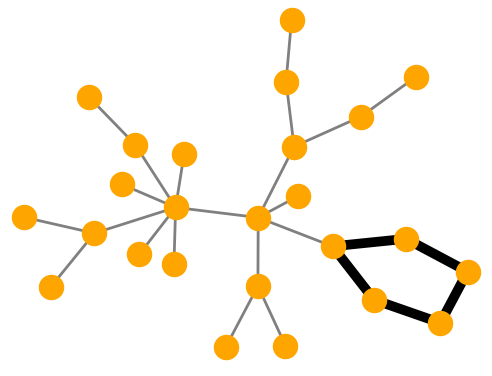
\includegraphics[width=.1\linewidth]{imgs/their_image-5.png} & 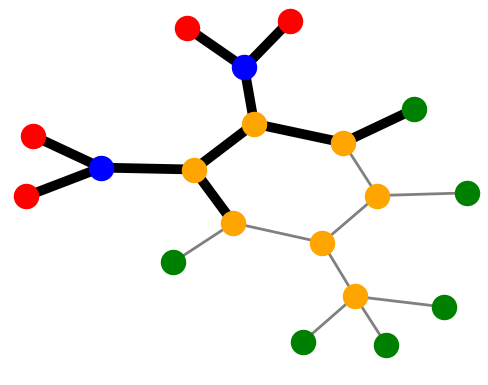
\includegraphics[width=.1\linewidth]{imgs/their_image-6.png} \\
% Reproduced & 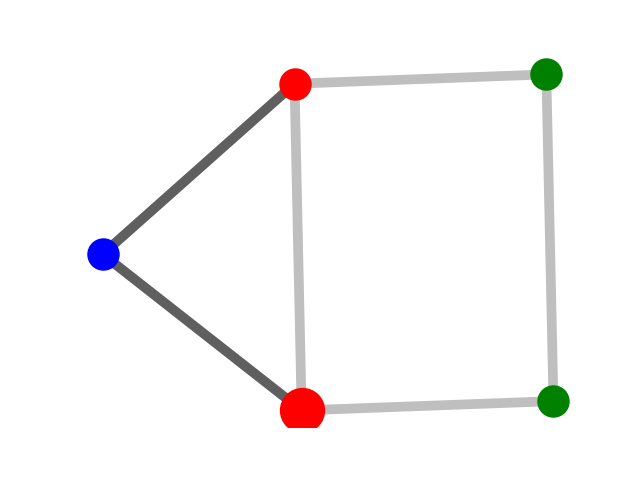
\includegraphics[width=.1\linewidth]{imgs/replication/syn1.png}
% & 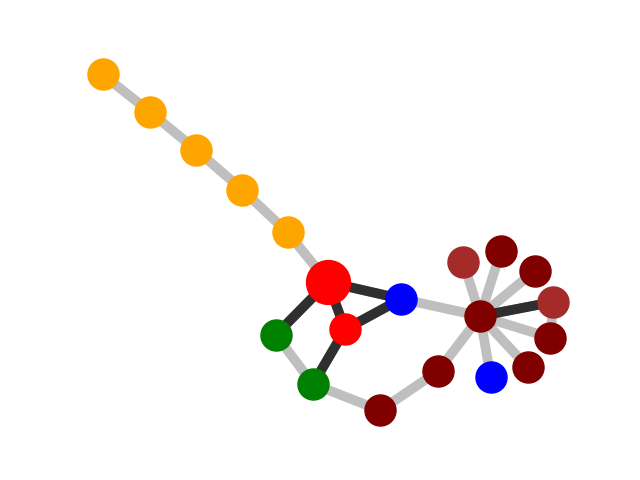
\includegraphics[width=.1\linewidth]{imgs/replication/syn2.png} & 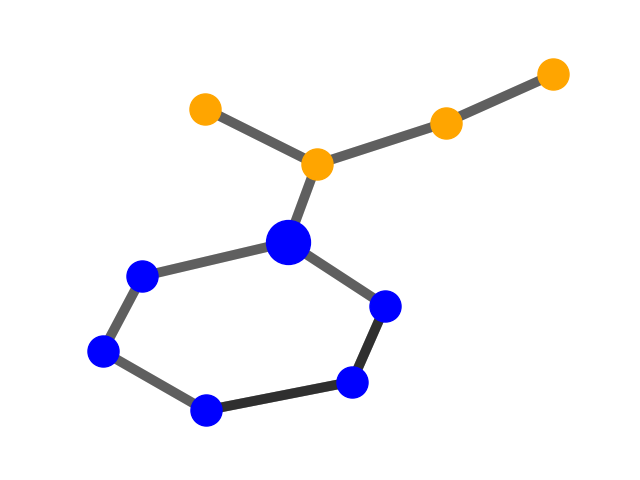
\includegraphics[width=.1\linewidth]{imgs/replication/syn3.png} & \multicolumn{1}{l|}{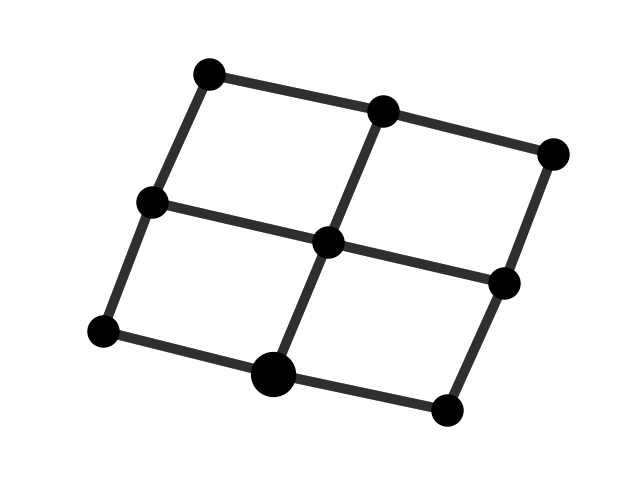
\includegraphics[width=.1\linewidth]{imgs/replication/syn4.png}} & img & 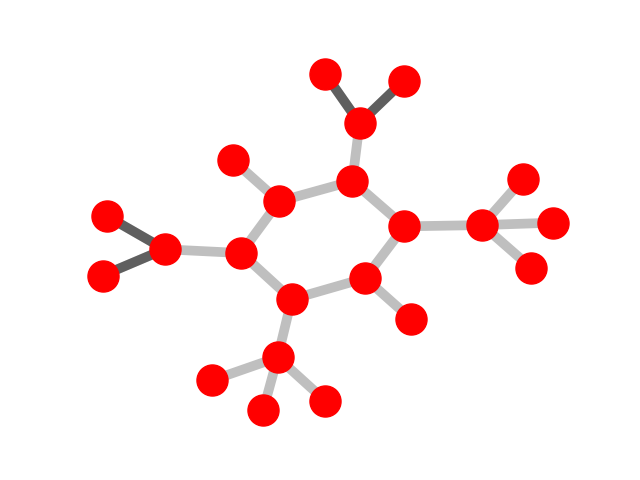
\includegraphics[width=.1\linewidth]{imgs/replication/85.png} \\ \hline
% \multicolumn{7}{l}{\textbf{Explanation AUC}} \\ \hline
% Original & 0.963 ± 0.011 & 0.945 ± 0.019 & 0.987 ± 0.007 & \multicolumn{1}{l|}{0.907 ± 0.014} & 0.926 ± 0.021 & 0.873 ± 0.013 \\ \hline
% Reproduced & 0.977 ± 0.006 & 0.970 ± 0.006 & 0.534 ± 0.186 & \multicolumn{1}{l|}{0.649 ± 0.045} & x.xx & 0.843 ± 0.084 \\ \hline
% \multicolumn{7}{l}{\textbf{Inference Time (ms)}} \\ \hline
% Reproduced & 3.56 & 5.29 & 0.40 & \multicolumn{1}{l|}{0.47} & x.xx & 2.09 \\ \bottomrule
% \end{tabular}
% \caption{Reproduction results}
% \label{tab:reproduction_results}
% \end{table}

% \paragraph{Qualitative}
% The replicated qualitative evaluation is very similar to the original results. PGExplainer is very capable of finding the motifs in the graphs and highlighting their edges. 

% \paragraph{Quantitative}
% The replicated quantitative evaluation shows results that are significantly different from the originals. Interestingly, the difference occurs in a different dataset then where the difference was observed in model accuracy. Despite the difference in validation and test accuracy between the replicated and the original model that is explained, the AUC score of the PGExplainer is very similar. On the other hand, the replicated evaluation of the tree-based graphs scores significantly lower, despite having very sensible qualitative explanations. One potential reason for this is the entropy and size regularization used in the PGExplainer. The configuration provided by the original codebase differ from the other datasets significantly for the tree-based datasets.

% \paragraph{Efficiency}
% Despite being evaluated using a considerably less powerful machine, and without utilizing a GPU, our implementation greatly outperforms the original implementation. 

% \subsection{Discussion}
% Based on the paper alone it is impossible to replicate the results presented in the paper, even if the complications of the evaluation itself are ignored. However, as the results presented above show, even with the provided codebase replicating the presented results is still not possible. First, the code base is badly structured and does not contain a central place describing the used configurations for training the models. Because of this a number of things remained unclear about the configuration of the models that might have lead to the reduced accuracy. For example, the training script configuration contained the possibility to use weight sharing and dropout to prevent over-fitting, but this is not used in any of the models. We hypothesize that this might be used for improving the accuracy of the BA-community model. 

% The replicated quantitative, qualitative and efficiency experiments similarly show that it is hard to reproduce the results prevented in the paper. Again, the main configuration files required to faithfully replicate the main results are missing. We believe that this effect is worsened by the crucial role of badly documented hyper parameters such as the entropy and size regularization coefficients. In the qualitative evaluation we expect that the importance of these hyper-parameters is hidden by the handpicked number of edges show in the explanation. The effect of these parameters will be further explored in the extended reproduction.

